% Jain Streeter -- technical report
% Compile with XeLaTeX (twice). Fonts: CMU (cm-unicode), shipped with TeX Live.
\documentclass[11pt,a4paper]{article}

\usepackage[a4paper,top=25mm,bottom=25mm,left=24mm,right=24mm,headheight=14pt]{geometry}
\usepackage{fontspec}
\usepackage{amsmath,amssymb,amsthm}
\usepackage{xcolor,graphicx}
\usepackage{booktabs,tabularx,array,longtable,multirow}
\usepackage{enumitem,caption,subcaption,float}
\usepackage{titlesec,fancyhdr}
\usepackage[hidelinks]{hyperref}

% ---------- fonts: CMU Serif text, CMU Sans Serif headings, CMU Typewriter code
\setmainfont{cmunrm.otf}[BoldFont=cmunbx.otf, ItalicFont=cmunti.otf, BoldItalicFont=cmunbi.otf]
\setsansfont{cmunss.otf}[BoldFont=cmunsx.otf, ItalicFont=cmunsi.otf, BoldItalicFont=cmunso.otf]
\setmonofont{cmuntt.otf}[BoldFont=cmuntb.otf, ItalicFont=cmunit.otf]

\definecolor{linkblue}{HTML}{1F4E9C}
\hypersetup{colorlinks=true,urlcolor=linkblue,linkcolor=black,citecolor=linkblue}

\newcommand{\repo}{https://github.com/PriyanshuIITGHY2006/InterIIT_Quant_Jain-Streeter}
\newcommand{\src}[2]{\href{\repo/blob/master/#1}{#2}}
\newcommand{\file}[1]{\href{\repo/blob/master/#1}{\texttt{\detokenize{#1}}}}

% ---------- layout
\setlength{\parindent}{0pt}
\setlength{\parskip}{5pt plus 1pt}
\linespread{1.05}
\setlist{nosep,leftmargin=16pt,itemsep=2pt,topsep=3pt}
\captionsetup{font=small,labelfont=bf,justification=justified,singlelinecheck=true,skip=5pt}
\renewcommand{\arraystretch}{1.15}
\newcolumntype{L}{>{\raggedright\arraybackslash}X}
\newcolumntype{R}[1]{>{\raggedleft\arraybackslash}p{#1}}
\setcounter{tocdepth}{2}
\renewcommand{\topfraction}{0.9}\renewcommand{\bottomfraction}{0.8}\renewcommand{\textfraction}{0.08}\renewcommand{\floatpagefraction}{0.75}\setcounter{topnumber}{3}\setcounter{totalnumber}{5}

\titleformat{\section}{\sffamily\bfseries\Large}{\thesection}{0.8em}{}
\titleformat{\subsection}{\sffamily\bfseries\large}{\thesubsection}{0.8em}{}
\titleformat{\subsubsection}{\sffamily\bfseries\normalsize}{\thesubsubsection}{0.8em}{}
\titlespacing*{\section}{0pt}{14pt}{6pt}
\titlespacing*{\subsection}{0pt}{10pt}{4pt}
\titlespacing*{\subsubsection}{0pt}{8pt}{2pt}

\pagestyle{fancy}
\fancyhf{}
\fancyhead[L]{\small\sffamily Jain Streeter \textperiodcentered{} Technical report}
\fancyhead[R]{\small\sffamily\nouppercase{\leftmark}}
\fancyfoot[L]{\small\href{\repo}{github.com/PriyanshuIITGHY2006/InterIIT\_Quant\_Jain-Streeter}}
\fancyfoot[R]{\small\thepage}
\renewcommand{\headrulewidth}{0.4pt}
\renewcommand{\sectionmark}[1]{\markboth{\thesection\quad #1}{}}

\theoremstyle{definition}
\newtheorem{proposition}{Proposition}
\newcommand{\fig}[3][0.92\linewidth]{%
  \begin{figure}[htbp]\centering\includegraphics[width=#1]{fig/#2}\caption{#3}\end{figure}}

\begin{document}

% =====================================================================
% TITLE PAGE
% =====================================================================
\begin{titlepage}
\thispagestyle{empty}
\newgeometry{top=22mm,bottom=22mm,left=24mm,right=24mm}
% ---- logo band: both Inter IIT marks at matched optical size, centred on one axis
\begin{center}
\begin{tabular}{@{}c@{\hspace{10mm}}c@{\hspace{10mm}}c@{}}
\raisebox{-0.5\height}{
\includegraphics[height=12.5mm]{fig/cv_techmeet.png}} &
\raisebox{-0.5\height}{\rule{0.5pt}{16mm}} &
\raisebox{-0.5\height}{
\includegraphics[height=17mm]{fig/cv_bootcamp.png}}
\end{tabular}
\end{center}
\vspace{5mm}
\noindent\rule{\linewidth}{0.6pt}

\vspace{38mm}
{\sffamily\small\addfontfeature{LetterSpace=25}TECHNICAL REPORT\par}
\vspace{6mm}
{\sffamily\bfseries\fontsize{30}{37}\selectfont Calm-Trend Regime Strategies\\for BTC/USDT and ETH/USDT\par}
\vspace{7mm}
{\large Trend following with regime-based position sizing,\\backtested on Binance hourly data, 2021--2025\par}
\vspace{12mm}
\begin{tabular}{@{}c@{\hspace{9mm}}c@{}}
\raisebox{-0.5\height}{
\includegraphics[height=15mm]{fig/cv_btc.png}} &
\raisebox{-0.5\height}{
\includegraphics[height=17mm]{fig/cv_eth.png}}
\end{tabular}

\vfill
\noindent\rule{\linewidth}{0.6pt}\par\vspace{4mm}
\noindent\begin{minipage}[t]{0.5\linewidth}
{\sffamily\bfseries\large Team Jain Streeter\par}
\vspace{2mm}
Priyanshu Debnath\\
Kushagra Verma
\end{minipage}\hfill
\begin{minipage}[t]{0.46\linewidth}\raggedleft
{\sffamily\bfseries\large Inter IIT Tech Meet 15.0\par}
\vspace{2mm}
Inter IIT Bootcamp\\
Quant problem statement
\end{minipage}

\vspace{5mm}
\noindent{\small Code, data pipeline and all result files: \href{\repo}{github.com/PriyanshuIITGHY2006/InterIIT\_Quant\_Jain-Streeter}}
\restoregeometry
\end{titlepage}

\section*{Abstract}
We designed two daily trading strategies from one rule set and backtested them on Binance hourly candles for 2021--2025 with 10{,}000 USDT, 0.15\% cost per fill and next-open execution.
Our data research found that the direction of BTC and ETH is close to unpredictable at useful horizons, while the size of their moves is strongly predictable.
The strategies therefore use a slow, averaged trend signal to decide whether to hold and the market's volatility and trend-quality state to decide how much.
CTR-S (BTC) adds a half-size short only in calm, fully confirmed bear markets; CTR-ETH (ETH) is long only.
Over 2021--2025, CTR-S returned +368.4\% (buy-and-hold +197.9\%) with a maximum drawdown of $-29.6\%$ ($-76.6\%$), and CTR-ETH returned +481.7\% (+306.5\%) with $-37.3\%$ ($-79.3\%$).
This report documents the data analysis, the indicator, machine-learning and strategy research, the mathematics behind each rule, every idea we tested and rejected, the backtest engine, the risk plan and the results.

\vspace{4mm}
\tableofcontents
\newpage

% =====================================================================
\section{Introduction}
% =====================================================================
\subsection{The task}
The problem statement asks for a trading strategy on BTC/USDT and ETH/USDT, designed from data research, backtested over 1 January 2021 to 31 December 2025 and evaluated on 15 required metrics.
The fixed conditions are a starting capital of 10{,}000 USDT, a cost of 0.15\% of notional on every fill (fee and slippage, so a round trip costs 0.30\%), and decisions that can only be executed after the information they use is available.

\subsection{Approach in one paragraph}
We studied the data before writing any strategy (Sections~\ref{sec:data}--\ref{sec:eda}), tested more than 25 indicators and a set of machine-learning and reinforcement-learning models (Sections~\ref{sec:ind}--\ref{sec:ml}), and developed the strategy through a sequence of pre-registered stages in which most ideas failed (Section~\ref{sec:dev}).
The final design (Section~\ref{sec:strategy}) separates the two jobs a position has: a robust trend signal decides \emph{whether} to be long, flat or short, and the market's measured state decides \emph{how much}.
The same code is the BTC and the ETH strategy; every threshold is a rank within the coin's own history, so nothing was tuned per coin.

\subsection{Headline results, 2021--2025}
\begin{table}[htbp]\centering\small
\begin{tabularx}{0.95\linewidth}{@{}L R{19mm}R{19mm}R{19mm}R{19mm}@{}}
\toprule
 & \multicolumn{2}{c}{\textbf{BTC}} & \multicolumn{2}{c}{\textbf{ETH}}\\
\cmidrule(lr){2-3}\cmidrule(l){4-5}
 & CTR-S & Buy-and-hold & CTR-ETH & Buy-and-hold\\
\midrule
Total return & \textbf{+368.4\%} & +197.9\% & \textbf{+481.7\%} & +306.5\%\\
Sharpe ratio & \textbf{0.98} & 0.67 & \textbf{0.96} & 0.75\\
Maximum drawdown & \textbf{$-29.6\%$} & $-76.6\%$ & \textbf{$-37.3\%$} & $-79.3\%$\\
Worst calendar year & $-4.3\%$ (2025) & $-64.2\%$ (2022) & $-20.2\%$ (2022) & $-67.5\%$ (2022)\\
Quarters beating buy-and-hold & 11 of 20 & -- & 10 of 20 & --\\
Down quarters beating buy-and-hold & 8 of 9 & -- & 7 of 8 & --\\
\bottomrule
\end{tabularx}
\caption{Summary of the required 2021--2025 backtest. All result files are in \file{results/}; we re-ran both strategies from the raw candles and reproduced every file exactly.}
\end{table}

% =====================================================================
\section{Data and cleaning}\label{sec:data}
% =====================================================================
\subsection{Inventory}
The source is Binance spot klines from the public REST endpoint \texttt{/api/v3/klines}, for BTCUSDT and ETHUSDT, hourly, from 2021-01-01 00:00 to 2025-12-31 23:00 UTC.
Each candle carries open, high, low, close, base volume, quote volume, number of trades and taker-buy volume.
The raw files have 43{,}810 rows each; after completing the time grid there are 43{,}824 hours per coin.
Daily, 4-hour and processed hourly files are derived from the cleaned hourly data and split into train (2021--2023), validation (2024) and test (2025).

A candle is labelled by its \emph{open} time. Its open price is known at that moment; its high, low, close and volume only when it closes. A decision computed from bar $t$ can be executed no earlier than the open of bar $t+1$.

\subsection{Quality checks}
\begin{table}[htbp]\centering\small
\begin{tabularx}{\linewidth}{@{}p{45mm}L@{}}
\toprule
\textbf{Check} & \textbf{Result}\\
\midrule
Missing hours & 14 hours in 7 outages (longest 4 hours on 2021-08-13), identical in both coins\\
Hidden outage bars & 3 bars with zero or almost no trading (2021-02-11 03:00, 2021-04-25 04:00, 2023-03-24 12:00); the two with zero trades are flagged as outages\\
OHLC consistency, VWAP inside range, taker $\le$ volume, positive prices & all pass, 0 violations\\
Open versus previous close & median gap $\approx10^{-7}$; only 5 jumps above 0.1\% (max 0.34\%)\\
Daily bars rebuilt from hourly versus Binance daily & exact match\\
Extreme moves & all genuine: both coins move together on 2--25$\times$ normal volume; BTC-only spikes on 2021-01-29 (+11.6\%) and 2021-02-08 (+8.6\%) match the Musk and Tesla news\\
Huge wicks & genuine liquidation cascades (2021-05-19, 2021-12-04, 2025-10-10); kept\\
\bottomrule
\end{tabularx}
\caption{Data quality checks (\file{notebooks/01_data_research.ipynb}). Verdict: the data is trustworthy.}
\end{table}

\subsection{Cleaning pipeline}
\begin{table}[htbp]\centering\small
\begin{tabularx}{\linewidth}{@{}p{38mm}p{58mm}L@{}}
\toprule
\textbf{Step} & \textbf{Rule} & \textbf{Why}\\
\midrule
Sort, deduplicate & keep the first row per timestamp & exchange exports occasionally repeat rows\\
Validate OHLC & prices positive; high and low widened to bound open and close & a high below the close breaks range-based volatility\\
Complete the grid & every hour from first to last timestamp & indicators assume a regular clock\\
Fill gaps forward only & flat candle at the previous close, zero volume & interpolation would use the next price, which is future data\\
Flag outages & \texttt{is\_filled} for filled hours and for \texttt{trades == 0} & the engine never trades on them\\
Daily bars & \texttt{resample("1D", label="left", closed="left")} & a day is complete only at 00:00 UTC the next day\\
Realised measures & per day, from that day's hourly returns & intraday information known at the day's close\\
\bottomrule
\end{tabularx}
\caption{Cleaning steps (\file{src/data/preprocess.py}; the same rules for new data in \file{src/system/ingest.py}).}
\end{table}

\subsection{A structural break made by the exchange}
\fig[0.8\linewidth]{activity_over_time.png}{Daily volume, trades and average trade size. The shaded band is Binance's BTC zero-fee promotion (8 July 2022 -- 22 March 2023).}
During the zero-fee promotion BTC trades per day rose from 1.6 million to 6.3 million (3.8$\times$), volume doubled and the average trade size halved (1{,}687 to 870 USDT), while ETH, which had no promotion, declined.
When the promotion ended BTC activity fell below its earlier level, and the average trade size of both coins fell sharply again in late 2024--2025.
Absolute volume, trade count and trade size are therefore not stationary for reasons unrelated to price behaviour, and \textbf{no activity measure is used as a trading signal}.

% =====================================================================
\section{Exploratory data analysis}\label{sec:eda}
% =====================================================================
All statistics in this section use only the training years 2021--2023, so 2024 and 2025 remained out-of-sample checks.

\subsection{Distribution of returns}
\fig[0.85\linewidth]{prices.png}{BTC and ETH normalised to 1 on 2021-01-01 (log scale), and the ETH/BTC ratio.}

\begin{table}[htbp]\centering\small
\begin{tabular}{@{}lrr@{}}
\toprule
\textbf{2021--2023} & \textbf{BTC} & \textbf{ETH}\\
\midrule
Annualised volatility & $\sim$65\% & $\sim$85\%\\
Hourly excess kurtosis & 15.7 & 13.4\\
Daily excess kurtosis & 3.5 & 5.7\\
Hourly skew & $-0.19$ & $-0.59$\\
Tail index $\alpha$ (Hill, hourly) & 2.7--3.7 & 2.6--4.0\\
Student-$t$ degrees of freedom (daily) & 2.5 & 2.9\\
Moves above $4\sigma$, relative to a normal & $\sim$135$\times$ & $\sim$134$\times$\\
\bottomrule
\end{tabular}
\caption{Distribution statistics.}
\end{table}

\fig{return_distribution.png}{Standardised hourly returns against the normal density (log scale).}

The Hill estimator of the tail index from the $k$ largest absolute returns $X_{(1)}\ge\dots\ge X_{(k)}$ is
\begin{equation}
\hat\alpha=\Bigl(\frac1k\sum_{i=1}^{k}\ln X_{(i)}-\ln X_{(k)}\Bigr)^{-1}.
\end{equation}
With $\hat\alpha\approx3$ the variance is finite but $\mathbb{E}|r|^p<\infty$ only for $p<\alpha$, so the fourth moment is probably not.
Kurtosis estimates jump as data is added, and every threshold in our strategies is therefore a rank, a percentile or a median, never a z-score.
Log prices are non-stationary and returns are stationary in the mean (ADF and KPSS agree); return variance is not constant.

\paragraph{Discovery: jumps arrive in calm markets.}
Scaling hourly returns by past volatility normally lowers kurtosis by removing volatility clustering. Here it \emph{raises} it (BTC 15.7 to 24.7), for EWMA spans of a day, a week and a month.
The largest scaled shocks are 5\% hourly moves that arrive when recent hourly volatility was about 0.25\% (for example 2023-08-17 and 2023-08-29); removing five such hours halves the scaled kurtosis.
Volatility-targeted sizing therefore puts on its largest positions exactly where these jumps hit, which is why our strategies cap exposure at 1.5$\times$ regardless of how calm the market is, and why the engine fills stops at the open when a bar gaps through them.

\subsection{Behaviour changes through time}
\begin{table}[htbp]\centering\small
\begin{tabular}{@{}lrrrrrr@{}}
\toprule
 & \multicolumn{3}{c}{\textbf{BTC}} & \multicolumn{3}{c}{\textbf{ETH}}\\
\cmidrule(lr){2-4}\cmidrule(l){5-7}
Year & Return & Volatility & Max DD & Return & Volatility & Max DD\\
\midrule
2021 & +58\% & 81\% & $-55\%$ & +404\% & 109\% & $-60\%$\\
2022 & $-64\%$ & 64\% & $-67\%$ & $-67\%$ & 87\% & $-77\%$\\
2023 & +156\% & 44\% & $-22\%$ & +91\% & 47\% & $-28\%$\\
\bottomrule
\end{tabular}
\caption{Three training years, three different markets.}
\end{table}
\begin{figure}[htbp]\centering
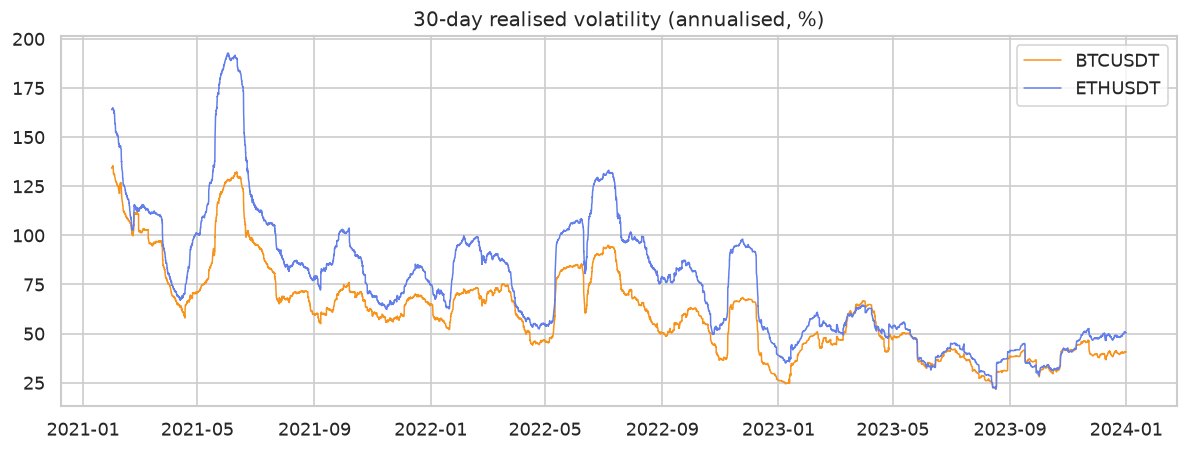
\includegraphics[width=0.49\linewidth]{fig/realised_vol.png}\hfill
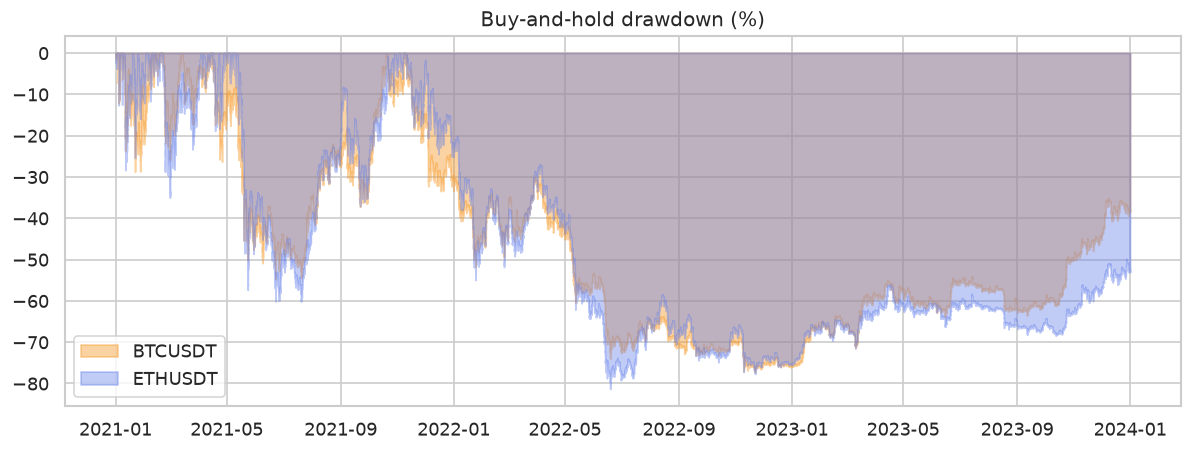
\includegraphics[width=0.49\linewidth]{fig/drawdowns.png}
\caption{Left: 30-day realised volatility. Right: buy-and-hold drawdown, 2021--2023.}
\end{figure}
Volatility halved from 2021 to 2023 (30-day volatility ranged 22--135\% for BTC and 22--193\% for ETH) and skew turned from negative to positive.
Buy-and-hold fell 77\% (BTC) and 81\% (ETH) and was still about 780 days under water at the end of 2023.
The market's character also changed: BTC's weekly variance ratio was 0.83 (mean-reverting) in 2021, 1.05 in 2022 and 1.34 (trending) in 2023.
A single fixed style, pure trend or pure mean reversion, is exposed to these changes.

\subsection{Memory: direction has none, size has a lot}
\fig[0.8\linewidth]{acf.png}{Autocorrelation of hourly returns (lags 1--48 h) and of absolute hourly returns (lags up to two weeks).}
The autocorrelation of returns is close to zero at all lags, and variance ratios are close to 1 at every horizon from 2 hours to 20 days.
The variance ratio is a weighted sum of autocorrelations,
\begin{equation}
\mathrm{VR}(q)=\frac{\operatorname{Var}\bigl(\sum_{i=1}^{q}r_{t+i}\bigr)}{q\operatorname{Var}(r_t)}=1+2\sum_{k=1}^{q-1}\Bigl(1-\frac kq\Bigr)\rho_k ,
\end{equation}
and the heteroskedasticity-robust Lo--MacKinlay estimates on daily BTC are 0.97, 1.00, 1.01 and 1.02 at $q=2,5,10,20$, all with $|z|<1$.
The size of moves, in contrast, has long memory: absolute returns stay autocorrelated for weeks with a 24-hour cycle, and the autocorrelation of log realised variance is 0.63--0.71 at one day and 0.26--0.33 at 90 days (Figure~\ref{fig:rvp}).
\begin{figure}[htbp]\centering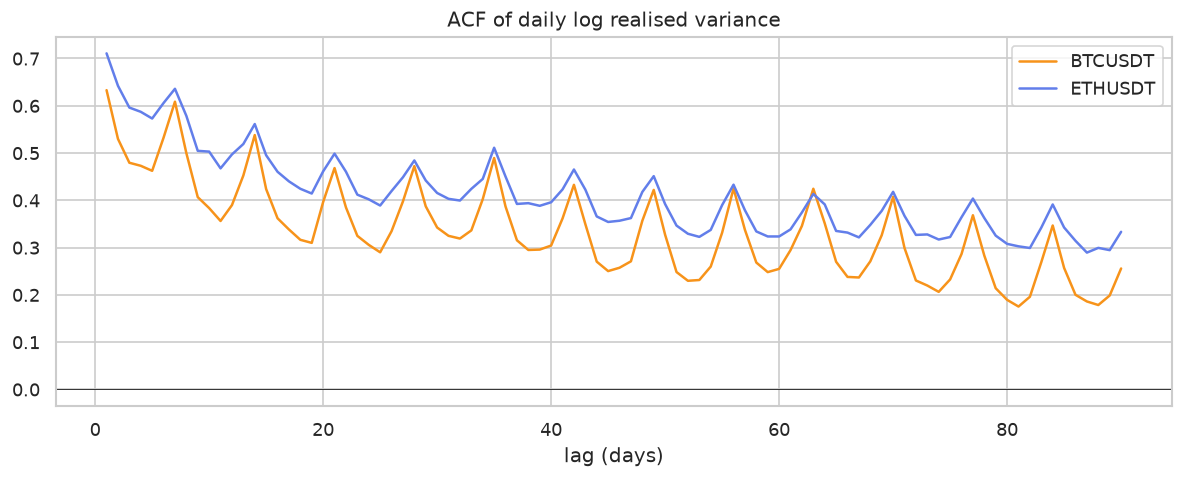
\includegraphics[width=0.62\linewidth]{fig/rv_persistence.png}\caption{Autocorrelation of daily log realised variance.}\label{fig:rvp}\end{figure}
Three further facts:
\begin{itemize}
\item The Spearman lag-1 autocorrelation is $-0.04$ to $-0.05$ while Pearson is $\approx0$: ordinary moves slightly reverse, the few huge ones do not, and they dominate Pearson.
\item There is no leverage effect. In GJR-GARCH(1,1), $h_t^2=\omega+\alpha r_{t-1}^2+\gamma r_{t-1}^2\mathbf 1\{r_{t-1}<0\}+\beta h_{t-1}^2$, the asymmetry term is insignificant ($p=0.95$ BTC, $0.68$ ETH): crypto volatility reacts about equally to up and down moves.
\item Fitted GARCH persistence is close to 1. This reflects the shifting volatility level rather than permanent shocks; one GARCH is mis-specified over this sample.
\end{itemize}

\paragraph{Volatility is forecastable out of sample.}
Corsi's heterogeneous autoregressive (HAR) model approximates long memory with three horizons,
\begin{equation}
\ln RV_{t+1}=\beta_0+\beta_d\ln RV^{(1)}_t+\beta_w\ln RV^{(5\text{--}7)}_t+\beta_m\ln RV^{(22\text{--}30)}_t+u_{t+1}.
\end{equation}
Fitted on 2021--22 (BTC: $\hat\beta_d=0.29$, $\hat\beta_w=0.51$, $\hat\beta_m=0.13$; ETH: 0.37, 0.47, 0.06), it explains 60\% (BTC) and 73\% (ETH) of next-day log volatility in 2023, with 34\% lower mean squared error than the forecast ``tomorrow equals today''. The weekly term dominates.

\subsection{BTC and ETH}
\fig[0.85\linewidth]{rolling_corr_beta.png}{Rolling 30-day correlation of hourly returns and rolling beta of ETH on BTC.}
\begin{table}[htbp]\centering\small
\begin{tabular}{@{}lr@{}}
\toprule
Correlation (1 h / 4 h / 1 d / 1 w) & 0.85 / 0.85 / 0.82 / 0.83\\
Rolling 30-day correlation range & 0.68 -- 0.95\\
ETH beta to BTC (mean, range) & 1.07 (0.71 -- 1.41)\\
Share of ETH variance explained by BTC & 68--73\%\\
Lead--lag at $\pm1$ hour & $\approx0$\\
\bottomrule
\end{tabular}
\caption{BTC--ETH co-movement.}
\end{table}
Dependence is asymmetric in the tails. For a quantile $q$ define the lower co-exceedance probability
\begin{equation}
\lambda_L(q)=\mathbb P\bigl(r^{ETH}\le F^{-1}_{ETH}(q)\mid r^{BTC}\le F^{-1}_{BTC}(q)\bigr)
\end{equation}
and $\lambda_U(q)$ with the inequalities reversed. On the worst and best 1\% of days $\lambda_L=0.82$ and $\lambda_U=0.27$, against 0.41 and 0.42 for a bivariate normal with the same correlation; the hourly figures (263 observations) point the same way (0.65 and 0.50).
The coins crash together and rally apart, so holding both gives diversification in rallies and none in crashes.

ETH/BTC ``mean reversion'' looked significant on the full sample (ADF $p=0.017$, cointegration $p=0.054$) but had ADF $p\ge0.19$ in every single year: the full-sample result is one round trip of the ratio. We dropped pairs trading.

\subsection{Seasonality}
\fig[0.6\linewidth]{hour_of_day.png}{Mean absolute hourly return, share of daily volume, and mean hourly return with 95\% intervals, by hour of day (UTC).}
Volatility and volume follow a stable daily cycle (peak at 14--15 UTC, about 30\% above average; trough at 04--06 UTC, about 25\% below), with year-to-year profile correlation 0.65--0.71.
Returns do not: the hourly return profile correlates $-0.16$ between years, one of 24 hours has $|t|>2$ (1.2 expected by chance), and no weekday has $|t|>1.1$. We use no calendar rule.

\subsection{Informative versus redundant variables}
\begin{table}[htbp]\centering\small
\begin{tabularx}{\linewidth}{@{}p{38mm}p{34mm}L@{}}
\toprule
\textbf{Variable} & \textbf{Informative about} & \textbf{Strength and notes}\\
\midrule
Last-hour high/low range & future volatility & IC 0.36--0.39 with the next 24 h absolute move, stable every year; best single variable\\
Past 24 h realised volatility & future volatility & IC 0.29--0.35, stable\\
Daily high/low (Parkinson) & next-day volatility & correlation 0.58--0.65, against 0.38--0.42 for the squared close return\\
Own 1--24 h returns & next 1--4 h direction (reversal) & IC $-0.04$ to $-0.07$, $t$ up to $-11$; economically too small (Section~\ref{sec:robfrag})\\
Taker buy ratio & same-hour return (mechanical) & next hour $-0.03$ to $-0.04$; mostly a proxy for the own return\\
Volume surprise & future volatility & IC 0.10--0.12 overall, but the sign flips between years\\
\texttt{log\_volume} vs \texttt{log\_trades} & -- & rank correlation 0.92: redundant\\
Amihud illiquidity & -- & rank correlation 0.68 with $|r|$: mostly the absolute return in disguise\\
\bottomrule
\end{tabularx}
\caption{What each variable carries information about.}
\end{table}
\fig[0.95\linewidth]{variable_correlations.png}{Rank correlations between the hourly variables.}

\subsection{Robust versus fragile relationships}\label{sec:robfrag}
\textbf{Robust.} Volatility clustering and its forecastability; the intraday volatility and volume cycle; fat tails and asymmetric crash dependence; and, statistically, short-term reversal: 33 of 78 predictive tests have $|t|>2$ (3.5 expected by chance) and 17 have $|t|>3$ (0.2 expected), with the same sign in all three years.

\textbf{Real but economically insufficient.} The reversal is far smaller than the 30 bps a round trip costs:
\begin{table}[htbp]\centering\small
\begin{tabular}{@{}lrr@{}}
\toprule
\textbf{Signal $\to$ target} & \textbf{Extreme-decile spread} & \textbf{Round-trip cost}\\
\midrule
BTC 4 h return $\to$ next 1 h & 2.3 bps & 30 bps\\
BTC 4 h return $\to$ next 4 h & 12.9 bps & 30 bps\\
ETH 4 h return $\to$ next 4 h & 14.6 bps & 30 bps\\
\bottomrule
\end{tabular}
\caption{The short-term reversal against costs.}
\end{table}
\fig{decile_curves.png}{Mean forward return by decile of the predictor.}

\textbf{Fragile.} ETH/BTC mean reversion (above); daily time-series momentum, where a 30-day lookback shows BTC +64\% a year but its 20-, 45- and 90-day neighbours are much weaker or negative and no lookback reaches $|t|=2$; volume surprise as a volatility predictor (sign flips by year); hour-of-day return effects; and BTC mean reversion in high-volatility regimes (a single test at $t\approx-2.6$).

\subsection{What the data told us}
\begin{enumerate}
\item \textbf{It is a volatility market more than a direction market.} The size of the next move is far more forecastable than its sign; sizing and risk management are where the clearest edge lies.
\item \textbf{Two coins, one factor.} ETH $\approx1.07\times$BTC plus independent noise, and the pair behaves as one asset in a crash.
\item \textbf{Regimes dominate.} Three years gave a bull, a bear and a recovery market with different volatility and different trend or reversion character.
\item \textbf{Danger comes out of calm.} The largest shocks relative to recent volatility arrive in quiet markets.
\item \textbf{Costs are large relative to short-horizon edges.} 30 bps per round trip removes every hourly effect found, so a viable strategy trades rarely and holds for days to months.
\item \textbf{Below the 200-day average}, next-day returns do not differ ($|t|\le1.1$) but volatility is higher (BTC 3.3\% against 2.7\% daily): a trend filter is a \emph{risk} switch, not a return signal.
\end{enumerate}

% =====================================================================
\section{Indicator research: why direction fails and volatility works}\label{sec:ind}
% =====================================================================
\subsection{Study design}
\file{notebooks/02_indicator_analysis.ipynb} tested more than 25 indicators in six families (volatility estimators, trend strength and choppiness, oscillators, squeezes, flow and liquidity, and filters and regime models from the literature).
Each was asked one question: \emph{does what it says hold in every year, for both coins?}
Predictive strength was measured by the rank information coefficient with next-week return, next-week volatility and next-week trend profit, year by year, with Newey--West standard errors for the overlapping 7-day targets.

\fig[0.66\linewidth]{ind_scorecard.png}{Indicator scorecard: yearly information coefficients of each indicator with next-week return (left) and with next-week volatility beyond current volatility (right), BTC (top) and ETH (bottom).}

\begin{table}[htbp]\centering\small
\begin{tabularx}{\linewidth}{@{}p{42mm}p{33mm}L@{}}
\toprule
\textbf{Family} & \textbf{Verdict} & \textbf{Evidence}\\
\midrule
Volatility level and forecasts & reliable & persistent every year; range-based estimators agree within a few percent\\
Downside semivariance & reliable & about 2$\times$ the forecasting weight of upside semivariance for BTC\\
Bipower variation & reliable & jumps fade within days; smooth volatility persists\\
Bollinger--Keltner squeeze & reliable for volatility only & volatility rises 10--14\% after a squeeze; the break direction is random\\
Choppiness $<38.2$, efficiency ratio & reliable as a trend-quality filter & trend payoff positive in clean trends in 4 of 4 years\\
RSI, stochastic RSI, Bollinger \%B, z-scores & unreliable for direction & the sign of the yearly IC flips; one exception: BTC bounced after RSI $<35$ in 4 of 4 years\\
ADX & unreliable for direction & measures trend strength, not sign\\
Supertrend, EMA ribbons, Heikin-Ashi, Kalman & no edge beyond a moving average & all are delayed linear filters of price\\
Hurst exponent & rejected & BTC's persistence matched shuffled data\\
CUSUM, Markov switching & variance classifiers & separate calm from stormy, not up from down\\
Amihud illiquidity & promising but caveated & IC $\ge0$ in 8 of 8 coin-years, but driven by volume drift and the zero-fee period\\
\bottomrule
\end{tabularx}
\caption{Indicator verdicts. The design rule that came out of this study: use reliable indicators to decide size, and the simplest robust trend measure to decide direction.}
\end{table}

\subsection{The model behind the verdicts}
Let $P_t$ be the daily close, $r_t=\ln P_t-\ln P_{t-1}$, and $\mathcal F_t$ the information available at the close of day $t$. Write
\begin{equation}
r_{t+1}=\mu_t+\sigma_t\varepsilon_{t+1},\qquad\mathbb E[\varepsilon_{t+1}\mid\mathcal F_t]=0,\quad\operatorname{Var}(\varepsilon_{t+1}\mid\mathcal F_t)=1.
\end{equation}
Section~\ref{sec:eda} showed that $\sigma_t$ is highly predictable and that $\mathbb E[r_{t+1}\mid\mathcal F_t]\approx\mu$, a constant. Every successful component of our strategy uses $\sigma_t$; every failed indicator tried to predict $\mu_t$.

\subsection{The information coefficient and the cost hurdle}
Let $s_t$ be an $\mathcal F_t$-measurable signal with information coefficient $\rho=\operatorname{corr}(s_t,r_{t+1:t+h})$. If $(s,r)$ is close to jointly Gaussian with $\mathbb E[r]=0$, the sign bet earns
\begin{equation}
\mathbb E[\operatorname{sign}(s)\,r]=\mathbb E\bigl[\operatorname{sign}(s)\,\mathbb E[r\mid s]\bigr]=\rho\,\frac{\sigma_r}{\sigma_s}\,\mathbb E|s|=\rho\,\sigma_r\sqrt{2/\pi}.
\end{equation}
Our strongest short-horizon effect, the 4-hour return predicting the next 4 hours, has $\rho\approx-0.07$. With $\sigma_{4h}=0.665/\sqrt{2190}\approx1.42\%$ the gross edge is about 7.9 bps per bet, against 30 bps of round-trip cost; the measured extreme-decile spread (13--15 bps) confirms the order of magnitude.
At portfolio level the fundamental law of active management, $\mathrm{IR}\approx\mathrm{IC}\sqrt{\mathrm{BR}}$, gives the same verdict: a weekly signal has breadth of about 52 bets a year, so $|\mathrm{IC}|\le0.05$ gives $\mathrm{IR}\le0.36$ before costs.
More generally, $N$ round trips a year with gross edge $e$ per trade earn roughly $N(e-0.30\%)$.

\subsection{Non-stationarity: an IC that changes sign}
Treat each year's IC as $\mathrm{IC}_y=\bar\kappa+u_y$ with $u_y\sim(0,\tau^2)$. For RSI, stochastic RSI, \%B, z-score, ADX, DI spread, Supertrend, EMA ribbon, Aroon, Heikin-Ashi, Kalman slope and CUSUM the yearly ICs change sign (Supertrend: $+0.11$, $-0.11$, $-0.04$, $-0.12$), so $\tau\gg|\bar\kappa|$ and a signal fitted in one regime is a coin flip in the next.

\subsection{Why each family of directional indicators fails}
\paragraph{Oscillators.} RSI is a bounded monotone transform of a ratio of Wilder averages, $\mathrm{RSI}_t=100-100/(1+RS_t)$ with $RS_t=\mathrm{EWMA}_{1/n}(r^+)_t/\mathrm{EWMA}_{1/n}(r^-)_t$. It is $\mathcal F_t$-measurable, so under the martingale-difference property $\mathbb E[r_{t+1}\mid\mathrm{RSI}_t]=\mathbb E\bigl[\mathbb E[r_{t+1}\mid\mathcal F_t]\mid\mathrm{RSI}_t\bigr]\approx\mu$ whatever its level. Overbought/oversold trading presumes $\rho_k<0$ at the oscillator's horizon; with $\mathrm{VR}\approx1$ there is none, and in trending years the sign reverses: RSI $>70$ was followed by gains in 2023--24 and losses in 2022.

\paragraph{ADX.} $\mathrm{DX}_t=100\,|DI^+_t-DI^-_t|/(DI^+_t+DI^-_t)$ is unchanged when the price path is reflected (up-moves and down-moves swap, so $DI^+\leftrightarrow DI^-$). It is an even function of direction and cannot carry directional information. Wilder smoothing is an EWMA with $\alpha=1/14$ and mean lag 13 bars, applied twice, so ADX reports trend strength about 26 bars after the move.

\paragraph{Moving averages and their relatives.} An $n$-day SMA has group delay $\tau_g=(n-1)/2$ days (99.5 days for $n=200$). To first order a linear trend rule holds $w_t=\sum_{k\ge0}a_kr_{t-k}$, so its expected profit is a weighted sum of autocovariances,
\begin{equation}
\mathbb E[w_tr_{t+1}]=\sum_{k\ge0}a_k\,\gamma(k+1).
\end{equation}
With $\gamma(k)\approx0$ this is close to zero while every sign change of $w$ costs $2c$. Fast filters flip more: a single 30-day rule made 59 trades in 2021--24 against 9 for the 100--250-day vote share, and its 50 trades shorter than 30 days lost 7{,}900 USDT. Slow filters pay only through rare, persistent autocorrelation episodes such as the multi-month 2023--24 trends.

\paragraph{Heikin-Ashi.} With $HA^c_t=(O_t+H_t+L_t+C_t)/4$ and $HA^o_t=\tfrac12(HA^o_{t-1}+HA^c_{t-1})$, unrolling gives $HA^o_t=\sum_{j\ge1}2^{-j}HA^c_{t-j}$, an EWMA with $\alpha=1/2$ of the lagged typical price. The candle colour is the sign of a very short momentum filter and inherits its zero expected profit.

\paragraph{Kalman filter.} For the local-level model $x_t=\ell_t+\varepsilon_t$ ($\operatorname{Var}=R$), $\ell_t=\ell_{t-1}+\eta_t$ ($\operatorname{Var}=Q$), the prior variance converges to $P=\bigl(Q+\sqrt{Q^2+4QR}\bigr)/2$ and the gain to $K=P/(P+R)$; the filtered level $\hat\ell_t=\hat\ell_{t-1}+K(x_t-\hat\ell_{t-1})$ is an EWMA. For our $Q/R=0.01$, $K=0.0951$: a 20-day exponential moving average.

\paragraph{CUSUM.} Page's $S^+_t=\max(0,S^+_{t-1}+d_t-k)$ is optimal for detecting a shift between known densities of i.i.d.\ observations. Here $d_t=\ln P_t-\hat\ell_t$ is an EWMA residual with autocorrelation about $1-K\approx0.9$, and the mean shift is negligible relative to $\sigma$; its bull/bear labels flip in predictive value year to year (ICs $+0.14$, $-0.11$, $+0.03$, $-0.08$).

\paragraph{Hurst exponent.} For independent data the expected rescaled range is not $cn^{1/2}$ but (Anis--Lloyd)
\begin{equation}
\mathbb E[R/S]_n=\frac{n-\frac12}{n}\,\frac{\Gamma\bigl(\frac{n-1}{2}\bigr)}{\sqrt\pi\,\Gamma\bigl(\frac n2\bigr)}\sum_{i=1}^{n-1}\sqrt{\frac{n-i}{i}},
\end{equation}
which over window sizes 8--64 implies a slope of 0.617 for pure noise. Our $\hat H=0.589$ on BTC is indistinguishable from the 0.594 measured on shuffled BTC returns: the apparent persistence is estimator bias.

\paragraph{Markov switching and HMMs.} The filtered recursion is $\alpha_t(j)\propto f_j(y_t)\sum_i\alpha_{t-1}(i)\Pi_{ij}$ and the predictive mean is $\sum_j\bigl(\sum_i\alpha_t(i)\Pi_{ij}\bigr)\mu_j$. Our fitted states have $\mu_j\approx0.000$ and $0.001$ per day but volatility levels of about 26\% and 66\% annualised, so the predictive mean is about zero whatever the probabilities. The model is a good volatility classifier (next-week volatility 0.59 against 0.47 across its states, persistence $\Pi_{11}=0.83$, $\Pi_{22}=0.90$) with no first-moment information.

\paragraph{PCA and K-means.} Lloyd's algorithm minimises $\sum_i\lVert x_i-c_{k(i)}\rVert^2$. With power-law features the second moment is dominated by a few extreme observations, centroids absorb the tails, and 90.5\% (BTC) and 93.5\% (ETH) of days collapse into one cluster: the clustering separates outliers from everything else.

\fig[0.85\linewidth]{nb02_07.png}{BTC with the reference report's price filters and CUSUM regime, in their causal versions (notebook 02).}

\subsection{Why the volatility side works}
\paragraph{Realised measures.} For a jump-diffusion $d\ln P_t=\mu_tdt+\sigma_tdW_t+dJ_t$ and hourly returns $r_{t,i}$ of day $t$,
\begin{gather}
RV_t=\sum_{i=1}^{M}r_{t,i}^2\;\longrightarrow\;\int_{t-1}^{t}\sigma_s^2ds+\sum_{t-1<s\le t}(\Delta J_s)^2,\\
BV_t=\frac{\pi}{2}\sum_{i=2}^{M}|r_{t,i}|\,|r_{t,i-1}|\;\longrightarrow\;\int_{t-1}^{t}\sigma_s^2ds,\qquad RS^{\pm}_t=\sum_i r_{t,i}^2\mathbf 1\{r_{t,i}\gtrless0\}.
\end{gather}
Bipower variation removes the jumps (Barndorff-Nielsen and Shephard), so $RV-BV$ isolates them, and the realised semivariances split $RV$ by sign. Regressing next week's variance on the parts gives:
\begin{table}[htbp]\centering\small
\begin{tabular}{@{}lr@{}}
\toprule
\textbf{Component} & \textbf{Coefficient on next week's variance}\\
\midrule
smooth (bipower) & 0.58\\
jump & 0.08\\
downside semivariance & 0.45\\
upside semivariance & 0.21\\
\bottomrule
\end{tabular}
\caption{Smooth risk persists, jumps fade, and bad volatility persists about twice as much as good.}
\end{table}
\fig[0.95\linewidth]{nb02_02.png}{Share of daily variance from jumps, and realised kurtosis of hourly returns (notebook 02).}

\paragraph{Range-based estimators.} Parkinson's $\hat\sigma^2=(\ln H/L)^2/(4\ln2)$ correlates 0.58 with next-day realised variance, against 0.38 for the squared daily return and 0.62 for hourly RV. Garman--Klass, Rogers--Satchell and Yang--Zhang estimates agreed within a few percent (Figure~\ref{fig:volest}). This is why the strategy's volatility percentile uses Parkinson volatility and why it still works on daily candles alone.
\begin{figure}[htbp]\centering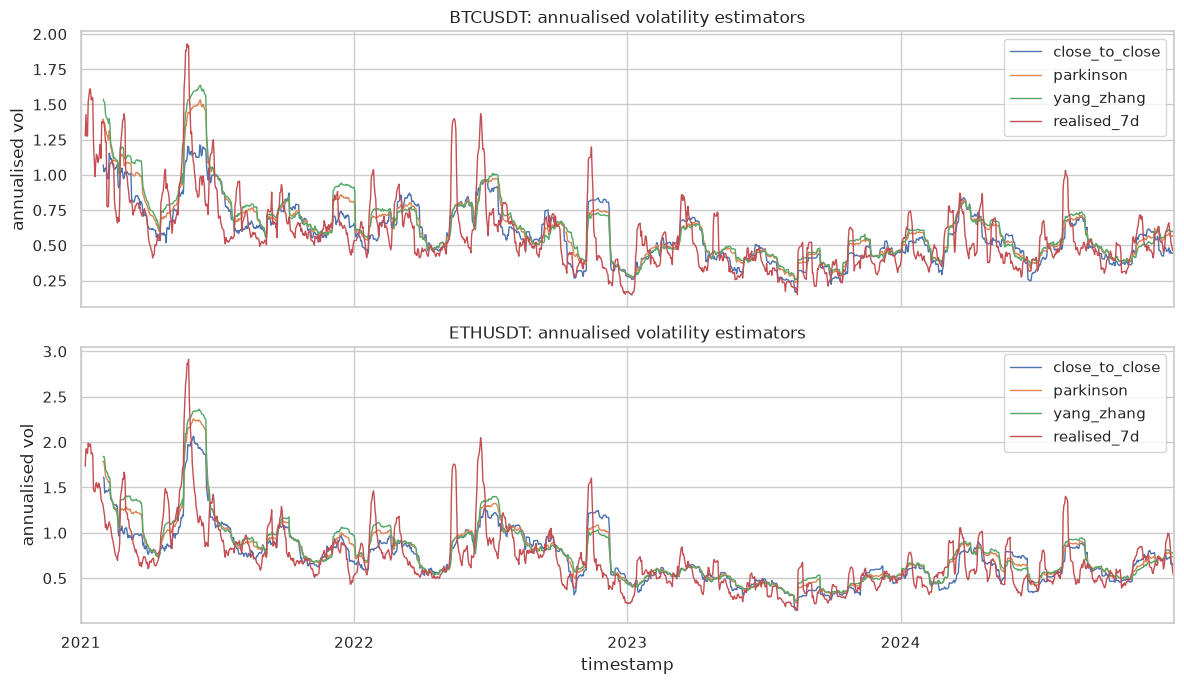
\includegraphics[width=0.8\linewidth]{fig/nb02_01.png}\caption{Annualised volatility estimators (notebook 02).}\label{fig:volest}\end{figure}

\begin{proposition}[Volatility-managed exposure raises the Sharpe ratio]
Assume $r_{t+1}=\mu+\sigma_t\varepsilon_{t+1}$ with $\sigma_t$ known at $t$ and $\varepsilon$ i.i.d.\ $(0,1)$ independent of $\sigma_t$. Constant exposure has $SR_0=\mu/\sqrt{\mathbb E[\sigma_t^2]}$. For $w_t=c/\sigma_t$,
\[
\mathbb E[w_tr_{t+1}]=c\mu\,\mathbb E[\sigma_t^{-1}],\qquad\operatorname{Var}(w_tr_{t+1})=c^2\bigl(1+\mu^2\operatorname{Var}(\sigma_t^{-1})\bigr).
\]
On daily data $\mu^2\operatorname{Var}(\sigma^{-1})\approx0$, and Jensen's inequality applied to $x\mapsto1/x$ and to $\sqrt{\cdot}$ gives
\begin{equation}
SR_{\text{managed}}\approx\mu\,\mathbb E[\sigma_t^{-1}]\ \ge\ \frac{\mu}{\mathbb E[\sigma_t]}\ \ge\ \frac{\mu}{\sqrt{\mathbb E[\sigma_t^2]}}=SR_0.
\end{equation}
\end{proposition}
The condition is that $\mu$ is roughly independent of $\sigma_t$; for BTC, mean returns do not differ across volatility terciles (all $|t|<1.5$). In our ablation the volatility layer moved the Sharpe ratio from 0.99 to 1.06 and cut the maximum drawdown from $-47\%$ to $-38\%$.

\paragraph{Trend quality against a random walk.} The efficiency ratio $ER_n=|P_t-P_{t-n}|/\sum_{i=1}^{n}|\Delta P_{t-i+1}|$ has, for a driftless Gaussian walk, $\mathbb E|S_n|=\sigma\sqrt{2n/\pi}$ and $\mathbb E\sum|\Delta P|=n\sigma\sqrt{2/\pi}$, so $\mathbb E[ER_n]\approx1/\sqrt n=0.183$ at $n=30$; simulation gives 0.183--0.187 and BTC averages 0.213. The choppiness index $CI_n=100\log_{10}\bigl(\sum TR/(\max H-\min L)\bigr)/\log_{10}n$ tends to about 50 for a random walk; simulation gives 47.2 and BTC averages 49.7. Choppiness is BTC's normal state, and $CI<38.2$ marks paths markedly straighter than chance (14\% of days).

\paragraph{Trend pays only in calm, orderly markets.} Splitting days by volatility and trend efficiency, a 30-day momentum bet earned money in calm trends in 4 of 4 years and roughly nothing in high-volatility regimes; on ETH the low-volatility trending regime paid +2.3\% per week on average. Choppiness below 38.2 also paid in 4 of 4 years.
\fig[0.8\linewidth]{nb02_06.png}{BTC and ETH coloured by four regimes: high-volatility trend, high-volatility chop, low-volatility trend, low-volatility chop (notebook 02).}

\paragraph{The squeeze.} When the Bollinger Bands sit inside the Keltner Channel, volatility rises 10--14\% over the following days but the direction of the break is random, so the right response is to cut size, not to bet on a breakout.
\fig[0.8\linewidth]{nb02_03.png}{Days in a Bollinger--Keltner squeeze (notebook 02).}

% =====================================================================
\section{Machine-learning and reinforcement-learning research}\label{sec:ml}
% =====================================================================
A separate study tested whether machine learning could find what the rules missed. It used 2021--2023 data only, monthly walk-forward training with an 8--11 day embargo between training and test, settings fixed before any run, and shuffled-label placebos and constant-size controls.

\begin{table}[htbp]\centering\small
\begin{tabularx}{\linewidth}{@{}p{48mm}p{62mm}L@{}}
\toprule
\textbf{Idea} & \textbf{Out-of-sample result (2022--2023)} & \textbf{Verdict}\\
\midrule
Direction classifiers (logistic regression, random forest, gradient boosting; 28 features) & AUC 0.40--0.51; placebo 0.52; trading the predictions lost 22\% (BTC) and 82\% (ETH) & dropped\\
HAR + gradient boosting for volatility & significantly worse than plain HAR for BTC (Diebold--Mariano $p=0.005$), equal for ETH ($p=0.87$) & HAR kept\\
Hidden Markov model regimes & cleaner calm/stormy separation, strategy unchanged (Sharpe 0.86 vs 0.88) & descriptive only\\
Triple-barrier trade filter & AUC 0.37--0.47; its gain equalled a constant half-size control & rejected\\
Tabular Q-learning & $-79\%$ (BTC), $-83\%$ (ETH) across all five seeds & rejected\\
\bottomrule
\end{tabularx}
\caption{Machine-learning and reinforcement-learning results.}
\end{table}

\paragraph{Too few independent samples.} Overlapping $h$-day labels leave $n_{\text{eff}}\approx T/h$ independent observations: two years of daily data with $h=7$ gives about 100. The Hanley--McNeil standard error of an AUC $A$ near 0.5,
\begin{equation}
SE(\hat A)=\sqrt{\frac{A(1-A)+(n_1-1)(Q_1-A^2)+(n_0-1)(Q_2-A^2)}{n_1n_0}},\quad Q_1=\frac{A}{2-A},\ Q_2=\frac{2A^2}{1+A},
\end{equation}
is then about 0.058, so any AUC within $0.5\pm0.11$ is noise. Our daily models (0.40--0.51) all sit in that band; the hourly model (0.535, 95\% interval 0.496--0.577) sits at its edge while the placebo reached 0.512--0.52. ETH's random forest was significantly worse than chance (0.40, interval 0.34--0.47). When the signal-to-noise ratio is this low the Bayes error dominates and extra capacity only adds variance, which is why gradient boosting lost to the linear HAR model.

\paragraph{Reinforcement learning.} Even with a generative model of the environment, learning an $\varepsilon$-optimal policy needs on the order of $\tilde O\bigl(|S||A|/((1-\gamma)^3\varepsilon^2)\bigr)$ samples. With $|S||A|=256$ and $\gamma=0.95$ this is about $2\times10^6/\varepsilon^2$ transitions, against 365 a year of data. Q-learning's convergence also needs stationary transition probabilities, which a regime-changing market violates. The agent memorised one bull year and held leverage into the 2022 crash.

The models learned the right economics (SHAP and partial-dependence plots show, for example, that the volatility model raises its forecast after downside semivariance), but with about three years of daily data they mostly fit noise. \textbf{No machine-learning or reinforcement-learning component is used by the final strategies.}

% =====================================================================
\section{Strategy development and rejected approaches}\label{sec:dev}
% =====================================================================
\subsection{Process discipline}
Look-ahead can also enter through the researcher. These rules applied throughout; each experiment's rules are recorded in the project's evaluation protocol.
\begin{table}[htbp]\centering\small
\begin{tabularx}{\linewidth}{@{}p{40mm}L@{}}
\toprule
Fixed splits & train 2021--2023, validation 2024, test 2025\\
Rules before results & every experiment's variants, gates and success criteria written down before it was run\\
Test once & a test period is evaluated once; a strategy is never changed after its test result\\
Validation becomes training & once a period has been used to select, it counts as training data\\
Ranges, not points & a parameter is accepted only if neighbouring values work too\\
Every trial logged & each backtest is appended to an experiment log; nothing is deleted\\
Luck benchmark & the deflated Sharpe ratio corrects for the number of trials (Section~\ref{sec:luck})\\
\bottomrule
\end{tabularx}
\caption{Evaluation protocol.}
\end{table}
2024 under-performed as a validation year for the first candidates and then became training data. 2025 was used once as the test of an early candidate (K-01: $-17.5\%$ against BTC's $-7.6\%$); later candidates were compared on it before the final choice, so 2025 is not an untouched test for the final strategy, and we say so.

\subsection{BTC: from baselines to CTR-S}
\begin{enumerate}
\item \textbf{Stages 1--9.} Baselines, trend ensembles, a regime gate and a chop filter led to K-01, frozen in protocol v6.
\item \textbf{Indicator research} (Section~\ref{sec:ind}): risk and regime indicators are reliable, direction indicators are not.
\item \textbf{Stages 10--10b.} First regime-sizing designs. B7 reached Sharpe 1.13 and +375\% but a $-51\%$ maximum drawdown.
\item \textbf{Stage 11.} The 2022 bear-market rallies were diagnosed as B7's weakness and K-01's soft 200-day gate was added. This design is CTR. It tied K-01 on Sharpe (1.1588 against 1.1556); CTR was chosen for +373\% against +289\% and 56\% against 50\% of quarters beating buy-and-hold, accepting a deeper drawdown.
\item \textbf{Stage 12.} The market-state framework. Refinements H1--H4 did not pass the cold-start gate, so CTR was unchanged.
\item \textbf{Stages 13--27.} A reliable-indicator baseline, a long-term direction study, a short-term layer, an ML risk engine, short-term and swing sleeves, and Bayesian regime-Kelly sizing. None beat CTR.
\item \textbf{Stages 28--31.} Rolling one-year windows over the full 2017--2026 history: CTR beat buy-and-hold in most bear windows but in only about 20\% of bull windows.
\item \textbf{Stage 32.} Four pre-registered short sides on top of CTR (Section~\ref{sec:short}); only X3 passed every gate.
\item \textbf{Stage 33.} X3 was checked year by year and adopted as the BTC final, CTR-S. The short-borrow fee, first applied after the fact, moved into the engine; the 2021--24 result is unchanged at reported precision (+388.85\% against +388.66\%).
\end{enumerate}

\subsection{Rejected approaches and why they failed}
\begin{longtable}{@{}p{50mm}p{50mm}p{50mm}@{}}
\toprule
\textbf{Idea (stage)} & \textbf{Result} & \textbf{Why it failed}\\
\midrule\endhead
\bottomrule\endfoot
Fixed 3$\times$ATR trailing stop (11) & fired 37 times; BTC Sharpe 1.16 $\to$ 0.71, return +373\% $\to$ +125\% & on daily crypto a price stop sells dips that recover, because jumps fade; under a random walk stops lower returns (Kaminski and Lo)\\
No leverage after a 15\% drawdown (11) & Sharpe 1.05, same maximum drawdown & lower Sharpe with no drawdown benefit\\
Smoother calm-trend label; downside-only brake (12) & Sharpe +0.01 / +0.02 & within noise; failed the cold-start gate\\
Leverage only on full trend agreement (12) & Sharpe 1.13, deeper drawdown & worse on both counts\\
No leverage when far above the 200-day average, or on volume surges (12) & dropped before testing & the leveraged days in question earned more, not less\\
Short-term dip-buying in an uptrend, rule-based and ML (15) & $-8.2\%$ and $-16.5\%$ while BTC rose 102.5\% (2022--24) & hit rate below break-even (Section~\ref{sec:breakeven})\\
ML/RL leverage control: quantile boosting, HMM, contextual bandit (16) & no better than the simple rules & no skill beyond a placebo\\
ML direction, triple-barrier filter, Q-learning & AUC $\le0.51$; Q-learning about $-79\%$ & inside the AUC noise band; RL sample complexity (Section~\ref{sec:ml})\\
Short-term and swing mean-reversion sleeves (25, 26) & edge per trade below the 0.30\% round trip & cost hurdle\\
Bayesian regime-Kelly sizing (27) & no gain over fixed regime sizes & needs an estimate of $\mu_t$, the least reliable input\\
1.5$\times$ above a banded 100-day average, else flat (31, 33) & maximum drawdown $-79.5\%$ over the longer history & $-77\%$ in the 2018 bear market alone\\
Volatility-targeted sizing (early stages) & average exposure 0.65--0.74 & positions too small in bull markets; replaced by regime sizing\\
Intraday seasonality: long BTC 22:00--24:00 UTC & +2.1 bps a day, $t=0.9$, negative in 2022 & hour profiles anti-correlated across years: data snooping\\
Intraday time-series momentum & about 365 round trips a year & about 110\% a year in costs\\
ETH/BTC pairs trading & ADF $p\ge0.19$ in every year & one round trip of the ratio\\
\end{longtable}

\subsection{Break-even hit rate for short-term trading}\label{sec:breakeven}
A trade with take-profit and stop at $\pm k\sigma$ and round-trip cost $c$ has
\begin{equation}
\mathbb E[\text{PnL}]=pk\sigma-(1-p)k\sigma-c=(2p-1)k\sigma-c\quad\Longrightarrow\quad p^*=\frac12+\frac{c}{2k\sigma}.
\end{equation}
With $k=1$, daily $\sigma\approx3\%$ and $c=0.30\%$, $p^*=0.55$. Our dip trades hit the target first in 24 of 49 decided cases ($\hat p=0.49$), so they had to lose. The ML filter would have needed to lift $p$ by 6 points, far beyond its AUC of 0.535.

\subsection{ETH: why no ETH-specific design survived}
\begin{table}[htbp]\centering\small
\begin{tabularx}{\linewidth}{@{}p{60mm}L p{12mm}@{}}
\toprule
\textbf{ETH-specific idea} & \textbf{Result (2021--24 unless stated)} & \textbf{Stage}\\
\midrule
Slow direction alone (200-day, vote share, breakout, golden cross, momentum) & best Sharpe 0.79, below buy-and-hold's 0.87; drawdowns 53--62\% & 18\\
E3: 200-day + full 1.5$\times$ when all votes agree + crash brake D1 & Sharpe 0.95, +371\%, but 6 of 16 quarters beating buy-and-hold, failed cold start; 2025 $-11.2\%$ & 20, 20c\\
Fixes for E3 (hysteresis, cold-start rules, early entry) & all worse (Sharpe 0.59--0.80) & 20b\\
Earlier ETH final G-06 & 2021--25 Sharpe 0.83, maximum drawdown $-56.7\%$ & 4e, 20c\\
BTC short side on ETH & every variant lowered Sharpe and deepened the drawdown & 32\\
\textbf{The BTC framework unchanged (CTR-ETH)} & \textbf{2021--25 Sharpe 0.96, +482\%, maximum drawdown $-37.3\%$} & 12, 20c\\
\bottomrule
\end{tabularx}
\caption{ETH candidates.}
\end{table}

\paragraph{Crash speed against filter delay.} A banded $n$-day state exits only when $P_t<\mathrm{SMA}_n(P)_t(1-b_t)$, and the SMA lags by $(n-1)/2$ days. From its 8 November 2021 top ETH fell 33.5\% before the 200-day state exited on 7 January 2022, so slow-only designs carried most of each crash (drawdowns 53--62\%).

\paragraph{The crash indicator D1 and regime concentration.} D1 is the ratio of a 72-hour EWMA of hourly downside semivariance to its trailing 90-day median,
\begin{equation}
D1_t=\frac{\mathrm{EWMA}_{72h}\bigl(r_h^2\mathbf 1\{r_h<0\}\bigr)_t}{\operatorname{median}_{90d}\bigl(\mathrm{EWMA}_{72h}(r_h^2\mathbf 1\{r_h<0\})\bigr)_t}.
\end{equation}
In its top decile next week's mean maximum drawdown was $-11.0\%$ against $-7.4\%$, and it caught 22\% of the worst-decile weeks (a lift of 2.2), but beyond current volatility its rank correlation with next-week downside volatility is about zero ($-0.04$, $+0.06$, $-0.19$, $-0.16$ by year): it is a thermometer, not a forecast, and the storm brake already uses the same mechanism.
E3 reached Sharpe 0.95, but removing its ability to lever up in the first 200 days cut its return from +371\% to +171\%:
\begin{equation}
R_{E3}=R_{\text{early 2021}}+R_{\text{rest}},\qquad R_{\text{early 2021}}/R_{E3}\ \text{large},
\end{equation}
a sign of performance concentrated in one regime. E3 then lost 11.2\% in 2025 while CTR-ETH made 54.9\%.

% =====================================================================
\section{The final strategy}\label{sec:strategy}
% =====================================================================
\subsection{The market-state framework}
\file{src/strategies/market_state.py} reads any dataset the same way. From data up to each daily close it computes the trend votes, the 200-day gate, the volatility percentile, trend quality, the downside risk forecast and the squeeze flag, and names the market's state. Every threshold is relative to the data's own trailing history, and averages warm up adaptively, so the same code works on a new coin, period or price level from a cold start.

\begin{table}[htbp]\centering\small
\begin{tabularx}{\linewidth}{@{}p{24mm}L R{11mm}R{11mm}R{11mm}R{11mm}R{11mm}R{11mm}@{}}
\toprule
 & & \multicolumn{3}{c}{\textbf{BTC}} & \multicolumn{3}{c}{\textbf{ETH}}\\
\cmidrule(lr){3-5}\cmidrule(l){6-8}
\textbf{State} & \textbf{Definition (priority order)} & days & spell & long & days & spell & long\\
\midrule
Storm & risk forecast $>1.5\times$ its 1-year median & 4\% & 7 d & 0.15 & 7\% & 11 d & 0.10\\
Downtrend & gate down, $<$ half the votes up & 34\% & 31 d & 0.04 & 34\% & 27 d & 0.04\\
Bear rally & gate down, $\ge$ half the votes up & 5\% & 9 d & 0.38 & 7\% & 11 d & 0.40\\
Calm uptrend & gate up, votes up, calm and orderly & 20\% & 7 d & \textbf{1.42} & 15\% & 10 d & \textbf{1.38}\\
Volatile uptrend & gate up, votes up, stormy & 9\% & 6 d & 0.54 & 12\% & 9 d & 0.52\\
Uptrend & gate up, votes up, neither & 17\% & 7 d & 0.79 & 17\% & 10 d & 0.84\\
Fading uptrend & gate up, $<$ half the votes up & 10\% & 10 d & 0.27 & 9\% & 11 d & 0.26\\
\bottomrule
\end{tabularx}
\caption{Market states, 2021--2025: share of days, average spell length and average long exposure. States are persistent: unchanged the next day 83--97\% of the time.}
\end{table}
\fig[0.8\linewidth]{btc_states.png}{BTC 2021--2025, each day coloured by its market state.}
\fig[0.8\linewidth]{eth_states.png}{ETH 2021--2025, each day coloured by its market state.}

\subsection{The daily decision}
Evaluated at each daily close; the order fills at the next day's open.

\paragraph{1. Direction: seven banded trend votes.} For each $n\in\{20,30,50,75,100,150,200\}$, with daily volatility $\sigma_t=\sqrt{\mathrm{EWMA}_{60}(r_t^2)}$ as a hysteresis band,
\begin{equation}
V_{n,t}=\begin{cases}1 & P_t>\mathrm{SMA}_{n,t}(1+\sigma_t)\\0 & P_t<\mathrm{SMA}_{n,t}(1-\sigma_t)\\V_{n,t-1} & \text{otherwise,}\end{cases}\qquad\text{votes}_t=\frac17\sum_nV_{n,t}.
\end{equation}

\paragraph{2. Regime.} With $\pi_t$ the rank of 14-day Parkinson volatility within the trailing 365 days, $ER_t$ the 30-day efficiency ratio and $CI_t$ the 14-day choppiness index,
\begin{gather}
\pi_t=\frac{1}{365}\sum_{s=t-365}^{t-1}\mathbf 1\{\sigma^P_s<\sigma^P_t\},\\
\text{regime}_t=\begin{cases}1.5 & (\pi_t\le0.5\wedge ER_t>\operatorname{median}_{s\le t}ER_s)\vee CI_t<38.2\\0.6 & \pi_t>0.5\\1 & \text{otherwise.}\end{cases}
\end{gather}

\paragraph{3. Storm brake.} From hourly data,
\begin{equation}
F_t=\sqrt{365\cdot\mathrm{EWMA}_{30}\bigl(0.5\,BV_t+RS^-_t\bigr)},\qquad\text{brake}_t=\begin{cases}0.5 & F_t>1.5\cdot\operatorname{median}_{365}(F)_t\\1&\text{otherwise.}\end{cases}
\end{equation}

\paragraph{4. Squeeze.} $\text{squeeze}_t=0.75$ while the Bollinger Bands $\mathrm{SMA}_{20}\pm2\,\mathrm{sd}_{20}$ sit inside the Keltner Channel $\mathrm{EMA}_{20}\pm1.5\,\mathrm{ATR}_{20}$, else 1.

\paragraph{5. Long-term gate.} $\text{gate}_t=0.5+0.5\,V_{200,t}$.

\paragraph{Target.}
\begin{equation}
\boxed{\ \text{Long}_t=\min\bigl(\text{votes}_t\cdot\text{regime}_t\cdot\text{brake}_t\cdot\text{squeeze}_t,\ 1.5\bigr)\cdot\text{gate}_t\ }
\end{equation}
as a fraction of equity. Every parameter (the 20--200-day averages, the 0.5 median split, Choppiness 38.2, 1.5$\times$ leverage, the 30-day EWMA, half-size shorts, the $-60\%$ capitulation line) is a round or conventional value fixed before testing; none was optimised.

\subsection{Why each layer is there}
\begin{table}[htbp]\centering\small
\begin{tabularx}{\linewidth}{@{}p{30mm}L p{48mm}@{}}
\toprule
\textbf{Layer} & \textbf{Evidence (2021--24)} & \textbf{Without it}\\
\midrule
7 averaged votes & single 30-day rule: Sharpe 1.08; its 20- and 45-day neighbours 0.77 and 0.68 & whipsaw: 50 trades under 30 days lost 7{,}900 USDT\\
Calm-trend 1.5$\times$ & trend payoff positive in calm trends in 4 of 4 years; the 18.5\% of days above 1$\times$ earned most of the return & long-term votes alone: Sharpe 0.96, +252\%\\
Stormy 0.6$\times$ & momentum payoff about zero or negative in high volatility & stormy entries lost 3{,}700 USDT net\\
Downside storm brake & sell-off volatility persists about twice as much as rally volatility & a brake on all volatility also fires in rallies\\
Squeeze 0.75$\times$ & volatility rises 10--14\% after a squeeze & Sharpe 1.13 $\to$ 1.04\\
200-day soft gate & 2022's bear rallies were the ungated design's main loss ($-51\%$ drawdown) & 2022: $-34\%$ instead of $-16\%$\\
\bottomrule
\end{tabularx}
\caption{Ablation evidence for each layer.}
\end{table}

\paragraph{The vote ensemble.} If $K$ signals have common variance $\sigma^2$ and pairwise correlation $\rho$, their average has variance $\sigma^2\bigl(\rho+\frac{1-\rho}{K}\bigr)$: 74\% of a single signal's for $K=7$ and $\rho\approx0.7$. More important, the vote share moves in steps of $1/7$, so turnover and cost are a fraction of a binary rule's, and the position mixes group delays from 9.5 to 99.5 days instead of betting on one lag. This is why the result is insensitive to the exact lookbacks while a single 30-day rule is not.

\begin{proposition}[Rank thresholds calibrate the rule to each coin]
Let $X_t$ be any risk measure and $\pi_t(X)=\frac1N\sum_{s=t-N}^{t-1}\mathbf 1\{X_s<X_t\}$. For any strictly increasing $g$, $\pi_t(g(X))=\pi_t(X)$, because $g(X_s)<g(X_t)\Leftrightarrow X_s<X_t$ term by term.
\end{proposition}
``Stormy'' therefore means stormy for that coin at its own volatility level (85\% for ETH, 65\% for BTC) with no free parameter, and the same holds for the efficiency ratio against its own median and the storm brake against its own median. This is why the same code is the ETH strategy, and why nothing was tuned for ETH.

\paragraph{Kelly and the leverage cap.} The growth-optimal exposure $f^*_t=\mu_t/\sigma_t^2$ is largest in calm trends, where $\mu_t>0$ in 4 of 4 years and $\sigma_t$ is below its median. The 1.5$\times$ cap is a fractional-Kelly guard against estimation error in $\mu_t$, the least reliable quantity in the system.

\fig[0.8\linewidth]{btc_layers.png}{BTC 2021--2025: price, vote share, sizing layers and the resulting target exposure.}

\subsection{The BTC short side (CTR-S)}\label{sec:short}
CTR-S holds $-0.5\times$ equity only while all five conditions hold, and covers at the next open as soon as one fails:
\begin{table}[htbp]\centering\small
\begin{tabularx}{\linewidth}{@{}p{8mm}p{55mm}L@{}}
\toprule
 & \textbf{Condition} & \textbf{Why}\\
\midrule
a & the long target is 0 & the short never overrides or reduces a long\\
b & the 200-day gate is down & a bear market, not a dip in a bull market\\
c & all 7 trend votes are down & every horizon agrees; the first vote to turn up (usually the 20-day) covers\\
d & volatility percentile $\le0.5$ & orderly declines persist; violent markets squeeze shorts\\
e & BTC less than 60\% below its 365-day high & after capitulation rebounds are sharpest: negative extremes mean-revert more strongly (Corbet and Katsiampa)\\
\bottomrule
\end{tabularx}
\caption{Short-side conditions: the calm, fully confirmed, non-capitulation part of the Downtrend state, about 6\% of days.}
\end{table}
Four variants were written down before any was run, with gates set in advance: beat CTR's Sharpe and return on 2021--24 also at double costs, keep 80\% of the Sharpe at every neighbouring setting, win at least as many rolling one-year windows as CTR, and have more positive bear-market windows.
\begin{table}[htbp]\centering\small
\begin{tabular}{@{}llrrrl@{}}
\toprule
\textbf{Variant} & \textbf{Short side} & \textbf{Sharpe} & \textbf{Return} & \textbf{Max DD} & \textbf{Result}\\
\midrule
Long-only CTR & none & 1.159 & +373\% & $-37.5\%$ & baseline\\
X1 & $-0.5\times$ when a--d hold & 1.10 & +343\% & $-33.3\%$ & failed the Sharpe gate\\
X2 & $-1.0\times$ when a--d hold & 0.98 & +284\% & $-36.7\%$ & failed\\
\textbf{X3 = CTR-S} & $\mathbf{-0.5\times}$ \textbf{when a--e hold} & \textbf{1.163} & \textbf{+389\%} & $\mathbf{-29.6\%}$ & \textbf{passed every gate}\\
X4 & $-0.5\times$ without condition d & 0.95 & +261\% & $-40.3\%$ & failed\\
\bottomrule
\end{tabular}
\caption{Pre-registered short-side variants, 2021--2024.}
\end{table}
Over 2021--2025 the short side turned 2022 from $-16.1\%$ into $-1.1\%$, cut the maximum drawdown from $-37.5\%$ to $-29.6\%$ and the longest time under water from 723 to 496 days. It costs a few points in bull years (2021 $-13$, 2023 $-4$, 2024 $-5$ points) from shorts caught by fast reversals. The 15 short trades sum to +3.8\% of equity but net $-334$ USDT, because the 2022 gains came at low equity; their value is the path, since the 2023--24 bull market compounds from a higher base.

\fig[0.8\linewidth]{ctr_s_vs_ctr.png}{BTC 2021--2025: CTR-S with shorts, the long-only CTR and buy-and-hold (log scale).}

\subsection{ETH (CTR-ETH)}
CTR-ETH applies the same rules to ETH, long only. ETH's direction is as unpredictable as BTC's, its volatility is more predictable (HAR $R^2=0.73$), and trend-following paid in calm ETH trends in 4 of 4 years. The fast votes leave within days of a break, so exposure falls stepwise (6/7, 5/7, \dots) long before the slow state exits; this is why CTR-ETH's maximum drawdown is $-37\%$ while slow-only designs had about $-58\%$.
\fig[0.8\linewidth]{eth_layers.png}{ETH 2021--2025: price, vote share, sizing layers and target exposure.}

\subsection{Execution settings}
\begin{table}[htbp]\centering\small
\begin{tabularx}{\linewidth}{@{}p{45mm}p{40mm}L@{}}
\toprule
Fee + slippage & 0.15\% of notional per fill & a round trip costs 0.30\%\\
Fill price & next bar's open & the engine applies the lag\\
Maximum long / short & 1.5$\times$ / 0.5$\times$ equity & short for BTC only\\
Borrowed USDT & 8\% a year, daily & when the long exceeds equity\\
Borrowed BTC & 10\% a year, daily, on the short's value & assumed margin rate\\
Rebalance band & resize only if the target moves $>0.25$ & limits churn and cost\\
Re-entry cool-down & 5 days & after an exit, before re-entering the same side\\
\bottomrule
\end{tabularx}
\caption{Execution settings (\file{src/strategies/execution.py}).}
\end{table}

% =====================================================================
\section{Backtest engine and look-ahead control}
% =====================================================================
\subsection{Design}
The engine's one job is to answer honestly what a strategy would have earned trading only on information it had, after paying 0.15\% on every fill; every design choice favours correctness and pessimism over speed. Strategies compute their signals with vectorised pandas code and the engine executes them in a plain bar loop (\file{src/backtest/engine.py}). A strategy returns a target position per bar; the engine, not the strategy, applies the one-bar lag. A strategy is a position process $w_t$ that must be $\mathcal F_t$-adapted, and the portfolio return is
\begin{equation}
R_{t+1}=w_t\,r^{\text{open}}_{t+1}-c\,|w_t-w_{t-1}|-b\,(w_t-1)^+,\qquad c=0.0015,
\end{equation}
with $b$ the daily borrowing rate on leverage above 1.

\begin{table}[htbp]\centering\small
\begin{tabularx}{\linewidth}{@{}p{42mm}p{50mm}L@{}}
\toprule
\textbf{Event} & \textbf{Fill rule} & \textbf{Why}\\
\midrule
Entry, exit, reversal & next tradable bar's open & the earliest price available after the decision\\
Stop or trailing stop & at the stop if touched; at the open if the bar opens beyond it & the data has real gaps and 10--20\% wicks\\
Stop and target in one bar & stop assumed first & OHLC cannot tell which came first\\
Trailing level & best price up to the previous bar & avoids assuming the high came before the low\\
Outage bar & no fills; orders wait & \texttt{is\_filled} or \texttt{trades == 0}\\
End of data & closed at the last close, with a fee & every trade is closed and costed\\
\bottomrule
\end{tabularx}
\caption{Fill rules. Sharpe and Sortino use daily equity returns $\times\sqrt{365}$ with a zero risk-free rate; buy-and-hold enters at the first tradable open and pays the same costs.}
\end{table}

\subsection{Keeping look-ahead out}
\begin{itemize}
\item \textbf{Features.} Only trailing windows, \texttt{ewm}, non-negative shifts, expanding statistics and percentiles within trailing windows. Forbidden in any strategy: centred windows, back-fill, interpolation, two-sided filters, Kalman smoothers, smoothed HMM probabilities, zigzag labelling, Ichimoku's backward-shifted lines, and any full-sample statistic applied to earlier points.
\item \textbf{Data.} Gaps are filled forward only; realised measures for a day use only that day's hours; an unfinished last day is dropped before any decision.
\item \textbf{Signal truncation test} (\file{src/backtest/checks.py}). Signals are recomputed on data cut at six points between bar 300 and the end and must be identical to the full-data signals up to each cut; otherwise the test fails with the first differing timestamp.
\item \textbf{Backtest truncation test.} The backtest re-run up to a cut must reproduce every trade and equity value before the cut.
\item \textbf{Engine validation.} A hand-computed round trip (967.05 USDT), gap and same-bar tests, outage tests, the invariants equity $=$ cash $+$ position value and $\sum$ trade PnL $=$ equity change on real data, an always-long strategy reproducing buy-and-hold exactly, random signals on zero-drift prices costing exactly 0.30\% per round trip, and a deliberately cheating \texttt{shift(-1)} signal that the causality check catches.
\end{itemize}
Both truncation tests run in the test suite for both strategies and every indicator, and inside every run on new data.

% =====================================================================
\section{Risk management}
% =====================================================================
\begin{table}[htbp]\centering\small
\begin{tabularx}{\linewidth}{@{}p{28mm}L L@{}}
\toprule
\textbf{Control} & \textbf{BTC (CTR-S)} & \textbf{ETH (CTR-ETH)}\\
\midrule
Position size & $\le1.5\times$ long, only in calm trends; $\le0.6\times$ when stormy; $\le0.5\times$ short & $\le1.5\times$, only in calm ETH trends; never short\\
Sell-off protection & storm brake on downside volatility (twice the forecasting weight of upside) & storm brake on ETH's own hourly sell-off volatility, squeeze, 200-day gate\\
Long exit & trend-break stop: the position shrinks vote by vote and closes when all votes are down & same\\
Short exit & cover at the next open when any of a--e fails, usually the 20-day vote turning up & --\\
Long and short & never at once: the short exists only when the long target is exactly zero (tested) & --\\
Joint risk & \multicolumn{2}{p{110mm}}{ETH crashes with BTC on 82\% of the worst days; run together, the two strategies are one risk position in a crash.}\\
\bottomrule
\end{tabularx}
\caption{Risk controls.}
\end{table}

\subsection{Payoff, not accuracy}
With win rate $p$, average win $W$ and average loss $L$ as fractions of equity,
\begin{equation}
\mathbb E[\text{trade}]=pW-(1-p)L,\qquad p^*=\frac{L}{W+L}.
\end{equation}
\begin{table}[htbp]\centering\small
\begin{tabular}{@{}lrr@{}}
\toprule
\textbf{2021--2025} & \textbf{BTC (36 trades)} & \textbf{ETH (21 trades)}\\
\midrule
Win rate & 33.3\% & 23.8\%\\
Average win / average loss (equity) & +22.0\% / $-2.2\%$ & +56.0\% / $-2.4\%$\\
Payoff ratio & 10.0 : 1 & 23.4 : 1\\
Profit factor & 4.31 & 5.06\\
Break-even win rate $p^*$ & 9.1\% & 4.1\%\\
Largest losing trade (equity) & $-10.6\%$ (5 August 2024 crash) & $-8.3\%$\\
Longest winning trade & 290 days & 258 days\\
\bottomrule
\end{tabular}
\caption{Risk--reward measured on equity. Many small losses are cut quickly and a few large wins run for months.}
\end{table}

\subsection{Drawdown arithmetic and volatility drag}
Recovering from a loss $L$ needs a gain of $L/(1-L)$, and geometric growth satisfies $g\approx\mu-\tfrac12\sigma^2$.
\begin{table}[htbp]\centering\small
\begin{tabular}{@{}lrr@{}}
\toprule
\textbf{Series} & \textbf{Maximum drawdown} & \textbf{Gain to recover}\\
\midrule
BTC buy-and-hold & $-76.6\%$ & +327\%\\
BTC CTR-S & $-29.6\%$ & +42\%\\
BTC long-only CTR & $-37.5\%$ & +60\%\\
ETH buy-and-hold & $-79.3\%$ & +383\%\\
ETH CTR-ETH & $-37.3\%$ & +60\%\\
\bottomrule
\end{tabular}
\caption{The asymmetry of losses.}
\end{table}
At BTC's 65\% volatility the drag is about 21\% a year at full exposure and at ETH's 85\% about 36\%; halving exposure in storms cuts the drag on those days by three quarters. This asymmetry, not better prediction, is why both strategies end well ahead while capturing less of each bull market.

\subsection{Tail risk and known risks}
\begin{table}[htbp]\centering\small
\begin{tabular}{@{}lrr@{}}
\toprule
 & \textbf{BTC} & \textbf{ETH}\\
\midrule
Worst day & $-15.7\%$ (7 Sep 2021) & $-18.6\%$ (7 Sep 2021)\\
Worst 7 days & $-23.8\%$ & $-25.7\%$\\
Daily 95\% VaR / CVaR & $-2.6\%$ / $-4.6\%$ & $-3.5\%$ / $-5.9\%$\\
Deepest drawdown and recovery & $-29.6\%$; longest under water 496 days & $-37.3\%$; 828 days to recover\\
\bottomrule
\end{tabular}
\caption{Measured tail risk, 2021--2025.}
\end{table}
\begin{itemize}
\item \textbf{Shocks from calm markets} hit while the strategies hold up to 1.5$\times$.
\item \textbf{Short squeezes in bull-market dips}: June 2021 ($-5.9\%$ of equity), September 2023 ($-2.0\%$), September 2024 ($-2.2\%$).
\item \textbf{Lag in bull markets}: 2021 Q1 BTC +52\% against +103\%; ETH 2021 +175\% against +399\%.
\item \textbf{Cold start on ETH is weaker}: from scratch in 11 quarterly windows its mean Sharpe was 0.62 against buy-and-hold's 0.74.
\item \textbf{Borrow cost} for BTC is an assumed 10\% a year; shorts were held on about 6\% of days and cost 235 USDT over 2021--25.
\end{itemize}

% =====================================================================
\section{Results, 2021--2025}
% =====================================================================
One continuous run per coin: 10{,}000 USDT, 0.15\% per fill, next-open execution, financing included.

\begin{table}[htbp]\centering\small
\begin{tabular}{@{}lrr@{}}
\toprule
\textbf{Required metric} & \textbf{BTC (CTR-S)} & \textbf{ETH (CTR-ETH)}\\
\midrule
Gross profit (USDT) & 47{,}963.39 & 60{,}041.03\\
Net profit (USDT) & 36{,}839.51 & 48{,}168.68\\
Total closed trades & 36 (21 long, 15 short) & 21\\
Win rate & 33.33\% & 23.81\%\\
Maximum drawdown & $-29.56\%$ & $-37.34\%$\\
Gross loss (USDT) & $-11{,}123.88$ & $-11{,}872.35$\\
Average winning trade (USDT) & 3{,}996.95 & 12{,}008.21\\
Average losing trade (USDT) & $-463.49$ & $-742.02$\\
Buy-and-hold return & +197.92\% & +306.46\%\\
Largest losing trade (USDT) & $-3{,}950.76$ & $-3{,}360.95$\\
Largest winning trade (USDT) & 19{,}827.38 & 24{,}676.80\\
Sharpe ratio & 0.98 & 0.96\\
Sortino ratio & 1.60 & 1.53\\
Average holding duration & 41.6 days & 64.3 days\\
Maximum holding duration & 290 days & 258 days\\
\midrule
\textit{Total / annualised return} & \textit{+368.40\% / 36.16\%} & \textit{+481.69\% / 42.19\%}\\
\textit{Calmar ratio} & \textit{1.22} & \textit{1.13}\\
\textit{Exposure; fees; financing (USDT)} & \textit{82\%; 4{,}412; 1{,}194} & \textit{74\%; 3{,}223; 753}\\
\textit{Sharpe at double costs} & \textit{0.90} & \textit{0.91}\\
\textit{Buy-and-hold Sharpe / maximum drawdown} & \textit{0.67 / $-76.63\%$} & \textit{0.75 / $-79.30\%$}\\
\bottomrule
\end{tabular}
\caption{The 15 required metrics and extras (\file{results/btc/2021-2025/metrics.md}, \file{results/eth/2021-2025/metrics.md}).}
\end{table}

\fig[0.8\linewidth]{btc_equity.png}{BTC: CTR-S equity and drawdown against buy-and-hold (log scale).}
\fig[0.8\linewidth]{eth_equity.png}{ETH: CTR-ETH equity and drawdown against buy-and-hold (log scale).}

\subsection{Year by year}
\begin{table}[htbp]\centering\small
\begin{tabular}{@{}lrrrrrrr@{}}
\toprule
 & \multicolumn{4}{c}{\textbf{BTC}} & \multicolumn{3}{c}{\textbf{ETH}}\\
\cmidrule(lr){2-5}\cmidrule(l){6-8}
Year & CTR-S & CTR & BTC & CTR-S DD & CTR-ETH & ETH & DD\\
\midrule
2021 & +37.1\% & +49.9\% & +59.8\% & $-27.4\%$ & +175.0\% & +399.2\% & $-37.2\%$\\
2022 & \textbf{$-1.1\%$} & $-16.1\%$ & $-64.2\%$ & $-12.7\%$ & \textbf{$-20.2\%$} & $-67.5\%$ & $-22.5\%$\\
2023 & +80.8\% & +84.4\% & +155.6\% & $-20.5\%$ & +40.0\% & +90.8\% & $-26.2\%$\\
2024 & +99.6\% & +104.1\% & +121.3\% & $-29.6\%$ & +21.8\% & +46.3\% & $-33.6\%$\\
2025 & $-4.3\%$ & $-3.3\%$ & $-6.3\%$ & $-20.6\%$ & \textbf{+55.4\%} & $-11.0\%$ & $-25.0\%$\\
\bottomrule
\end{tabular}
\caption{One continuous run per coin, cut by calendar year (\file{results/btc/2021-2025/yearly.csv}).}
\end{table}

\subsection{Quarter by quarter}
\begin{longtable}{@{}lrrrr@{}}
\caption{Quarterly returns (\file{results/btc/2021-2025/quarterly.csv}, \file{results/eth/2021-2025/quarterly.csv}). Bold: the strategy beat buy-and-hold. CTR-S beat BTC in 11 of 20 quarters and in 8 of the 9 where BTC fell; CTR-ETH beat ETH in 10 of 20 and in 7 of the 8 where ETH fell.}\\
\toprule
Quarter & CTR-S & BTC & CTR-ETH & ETH\\
\midrule\endfirsthead
\toprule
Quarter & CTR-S & BTC & CTR-ETH & ETH\\
\midrule\endhead
\bottomrule\endfoot
2021Q1 & +52.1\% & +103.1\% & +16.2\% & +160.6\%\\
2021Q2 & \textbf{$-$22.0\%} & $-$40.3\% & \textbf{+38.9\%} & +18.6\%\\
2021Q3 & +3.0\% & +25.1\% & \textbf{+40.5\%} & +31.9\%\\
2021Q4 & \textbf{+12.2\%} & +5.5\% & +21.3\% & +22.5\%\\
2022Q1 & \textbf{+5.8\%} & $-$1.5\% & \textbf{$-$0.3\%} & $-$10.7\%\\
2022Q2 & \textbf{+3.8\%} & $-$56.2\% & \textbf{$-$4.8\%} & $-$67.4\%\\
2022Q3 & $-$6.5\% & $-$2.6\% & $-$8.6\% & +24.1\%\\
2022Q4 & \textbf{$-$3.7\%} & $-$14.8\% & \textbf{$-$8.0\%} & $-$10.0\%\\
2023Q1 & +38.0\% & +72.1\% & +20.7\% & +52.3\%\\
2023Q2 & +5.5\% & +7.0\% & $-$0.6\% & +6.2\%\\
2023Q3 & \textbf{$-$11.3\%} & $-$11.5\% & \textbf{$-$9.0\%} & $-$13.6\%\\
2023Q4 & +39.9\% & +56.8\% & +28.2\% & +36.6\%\\
2024Q1 & \textbf{+68.7\%} & +68.6\% & +59.6\% & +59.8\%\\
2024Q2 & \textbf{$-$8.5\%} & $-$11.9\% & $-$10.5\% & $-$5.7\%\\
2024Q3 & $-$17.4\% & +0.9\% & \textbf{$-$16.0\%} & $-$24.3\%\\
2024Q4 & \textbf{+56.6\%} & +47.8\% & +1.5\% & +28.3\%\\
2025Q1 & \textbf{$-$5.7\%} & $-$11.8\% & \textbf{$-$9.8\%} & $-$45.4\%\\
2025Q2 & +11.3\% & +29.8\% & +6.4\% & +36.4\%\\
2025Q3 & $-$0.3\% & +6.4\% & \textbf{+89.7\%} & +66.8\%\\
2025Q4 & \textbf{$-$8.5\%} & $-$23.1\% & \textbf{$-$14.7\%} & $-$28.3\%\\

\end{longtable}

\fig[0.8\linewidth]{btc_trades.png}{BTC trades on price, 2021--2025.}

\subsection{Robustness}
\begin{table}[htbp]\centering\small
\begin{tabularx}{\linewidth}{@{}p{32mm}L L@{}}
\toprule
\textbf{Check} & \textbf{BTC CTR-S} & \textbf{ETH CTR-ETH}\\
\midrule
Neighbouring settings (2021--24) & long side keeps $\ge96\%$ of the Sharpe (high-vol size, volatility threshold, storm brake, gate floor and gate lookback each moved both ways); worst short-side neighbour 1.14 against 1.16 & $\ge90\%$; worst 0.81 against 0.90 (gate floor 0.7)\\
Double costs (0.30\% per fill) & Sharpe 1.08 (2021--24), 0.90 (2021--25) & 0.85, 0.91\\
Daily candles only & 1.17 against 1.16 & 0.88 against 0.90\\
Cold start, 11 quarterly windows & mean Sharpe 1.49; drawdowns $-28\%$ to $-38\%$; beat buy-and-hold's Sharpe in 7 & mean 0.62 against buy-and-hold's 0.74; beat it in 5\\
\bottomrule
\end{tabularx}
\caption{Robustness checks.}
\end{table}

\subsection{How much of the result could be luck?}\label{sec:luck}
For $N$ independent zero-skill strategies tested over $T$ years the expected best Sharpe ratio is (Bailey and L\'opez de Prado)
\begin{equation}
\mathbb E\bigl[\max_{i\le N}\widehat{SR}_i\bigr]\approx\frac{1}{\sqrt T}\Bigl[(1-\gamma)\Phi^{-1}\bigl(1-\tfrac1N\bigr)+\gamma\,\Phi^{-1}\bigl(1-\tfrac{1}{Ne}\bigr)\Bigr],\qquad\gamma\approx0.5772,
\end{equation}
which at $T=4$ is 0.79, 1.27 and 1.63 for $N=10$, 100 and 1{,}000. About 1{,}000 BTC backtests were logged, but they are small variations of about a dozen design families, so the effective $N$ is 10--20 and the luck benchmark about 0.8--1.0. The case for the strategies therefore does not rest on the 2021--24 Sharpe ratio alone but on stable neighbours, consistency year by year and the cold-start runs, none of which a lucky pick produces.

% =====================================================================
\section{Limitations and further work}
% =====================================================================
\begin{itemize}
\item \textbf{Bull markets.} The strategies hold about 0.5--0.8$\times$ on average in bull years and lag strong rallies; they beat buy-and-hold over full cycles, not every year.
\item \textbf{Calm-market crashes.} Jumps often arrive from calm markets, where exposure can be 1.5$\times$.
\item \textbf{Sample size of the short side.} It traded 15 times in 2021--25; its gain rests mainly on one bear market.
\item \textbf{Correlation.} ETH and BTC crash together, so the two strategies are not diversified in a crash.
\item \textbf{2025 was seen.} It was used once as an early candidate's test and then for comparing candidates, so it is not an untouched test.
\end{itemize}
Data that would improve the analysis: perpetual futures funding rates and open interest, liquidation data, minute or tick trades and order-book depth, other exchanges, options implied volatility (Deribit DVOL), macro calendars, on-chain stablecoin and exchange flows, and pre-2021 history.

% =====================================================================
\section*{References}
\addcontentsline{toc}{section}{References}
% =====================================================================
\small
\begin{enumerate}[leftmargin=18pt,itemsep=1pt]
\item Anis, A., Lloyd, E. (1976). The expected value of the adjusted rescaled Hurst range of independent normal summands. \emph{Biometrika}.
\item Azar, M., Munos, R., Kappen, H. (2013). Minimax PAC bounds on the sample complexity of reinforcement learning with a generative model. \emph{Machine Learning}.
\item Bailey, D., L\'opez de Prado, M. (2014). The deflated Sharpe ratio. \emph{Journal of Portfolio Management}.
\item Barndorff-Nielsen, O., Shephard, N. (2004). Power and bipower variation with stochastic volatility and jumps. \emph{Journal of Financial Econometrics}.
\item Barndorff-Nielsen, O., Kinnebrock, S., Shephard, N. (2010). Measuring downside risk: realised semivariance. In \emph{Volatility and Time Series Econometrics}.
\item Corbet, S., Katsiampa, P. (2020). Asymmetric mean reversion of Bitcoin price returns. \emph{International Review of Financial Analysis}.
\item Corsi, F. (2009). A simple approximate long-memory model of realized volatility. \emph{Journal of Financial Econometrics}. \href{https://doi.org/10.1093/jjfinec/nbp001}{doi:10.1093/jjfinec/nbp001}
\item Diebold, F., Mariano, R. (1995). Comparing predictive accuracy. \emph{Journal of Business \& Economic Statistics}.
\item Engle, R., Granger, C. (1987). Co-integration and error correction. \emph{Econometrica}. \href{https://doi.org/10.2307/1913236}{doi:10.2307/1913236}
\item Glosten, L., Jagannathan, R., Runkle, D. (1993). On the relation between the expected value and the volatility of the nominal excess return on stocks. \emph{Journal of Finance}.
\item Grinold, R. (1989). The fundamental law of active management. \emph{Journal of Portfolio Management}.
\item Hamilton, J. (1989). A new approach to the economic analysis of nonstationary time series and the business cycle. \emph{Econometrica}.
\item Hanley, J., McNeil, B. (1982). The meaning and use of the area under a ROC curve. \emph{Radiology}.
\item Hill, B. (1975). A simple general approach to inference about the tail of a distribution. \emph{Annals of Statistics}. \href{https://doi.org/10.1214/aos/1176343247}{doi:10.1214/aos/1176343247}
\item Joe, H. (1997). \emph{Multivariate Models and Dependence Concepts}. Chapman \& Hall.
\item Kaminski, K., Lo, A. (2014). When do stop-loss rules stop losses? \emph{Journal of Financial Markets}.
\item Kaufman, P. (1995). \emph{Smarter Trading}. McGraw-Hill.
\item Kelly, J. (1956). A new interpretation of information rate. \emph{Bell System Technical Journal}.
\item Lo, A., MacKinlay, C. (1988). Stock market prices do not follow random walks: evidence from a simple specification test. \emph{Review of Financial Studies}. \href{https://doi.org/10.1093/rfs/1.1.41}{doi:10.1093/rfs/1.1.41}
\item L\'opez de Prado, M. (2018). \emph{Advances in Financial Machine Learning}. Wiley.
\item Moreira, A., Muir, T. (2017). Volatility-managed portfolios. \emph{Journal of Finance}. \href{https://doi.org/10.1111/jofi.12513}{doi:10.1111/jofi.12513}
\item Moskowitz, T., Ooi, Y. H., Pedersen, L. H. (2012). Time series momentum. \emph{Journal of Financial Economics}. \href{https://doi.org/10.1016/j.jfineco.2011.11.003}{doi:10.1016/j.jfineco.2011.11.003}
\item Page, E. (1954). Continuous inspection schemes. \emph{Biometrika}.
\item Parkinson, M. (1980). The extreme value method for estimating the variance of the rate of return. \emph{Journal of Business}.
\item Patton, A., Sheppard, K. (2015). Good volatility, bad volatility: signed jumps and the persistence of volatility. \emph{Review of Economics and Statistics}.
\item Watkins, C., Dayan, P. (1992). Q-learning. \emph{Machine Learning}.
\item Zarattini, C., Pagani, A., Barbon, A. (2025). Catching crypto trends. SSRN working paper.
\end{enumerate}
The full annotated list, with what we took from each source, is in \file{reports/glossary.md}.

\end{document}
